\section{Experimental Setup}

The setup of our triated methane calibration technique can be separated into three parts: the injection system, the tritiated methane source bottle, and the zirconium getter.

\subsection{The tritiated methane source}

The tritiated methane source bottle for our calibration technique consists of a 2250 cc stainless steel bottle which is filled with a mixture of tritiated methane and xenon.  This source bottle was prepared in three steps.  First, we prepared a xenon bottle that had similar pressure and purity to the LUX system.  We filled a 2250 cc stainless steel bottle with 1590 torr of xenon from the same dekryptonation and purity program which the LUX xenon came from. The purpose of this xenon was to serve as a carrier gas for the triaited methane.  The next step was to prepare a small amount of tritiated methane to mix with this dekryptonated xenon.  A reservoir of tritiated methane with an activity of 204 Bq/torr-cc was purchased from Moravek Biochemical.  The reservoir was frozen with liquid nitrogen, resulting in a vapor pressure of 10.4 $\pm$ 0.05 torr.  We then opened the frozen tritiated methane reservoir to a 1/4" VCR cross which was sealed with swagelok valves on each side.  This first expansion space had a total volume of 5.2 $\pm$ 0.9 cc. Next, we isolated the VCR cross from the triated methane reservoir and then opened it to a 501 $\pm$ 0.2 cc expansion volume.  We isolated the VCR cross a second time and then opened it up to a 53.2 $\pm$ 3.4 cc expansion volume.  The VCR cross was then isolated for a third time before opening it to a 10.5 $\pm$ 0.5 cc expansion volume.  After this final expansion the VCR cross was isolated and the remaining 0.016 $\pm$ 0.006 torr-cc of tritiated methane left within was mixed with the dekryptonated xenon inside the 2250 cc bottle via cryopumping.  The final result was a tritiated methane source which had an activity of 9.1e-7 $\pm$ 3.4e-7 Bq/torr-cc.

\begin{figure}[H]
\centering
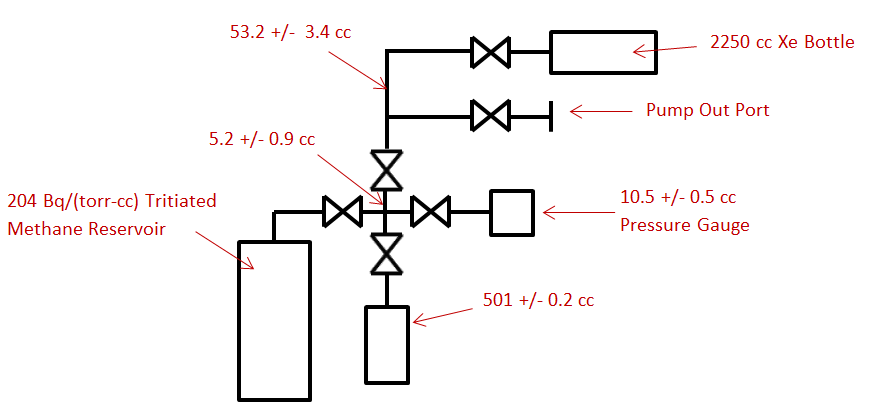
\includegraphics[scale=0.3]{BottleSetup.png}
\caption{The volume sharing system that was built to assemble our tritiated methane source bottle.}
\label{fig:BottleSetup}
\end{figure}


\subsection{The injection system}

The injection system for our tritiated methane calibration technique consists of a series of expansion volumes which are used to fine tune the amount of CH$_3$T that is injected.  Once the CH$_3$T source bottle is opened it flows through a methane gas purifier (SAES MC1-905F) to remove any sources of potential contamination, such as bare tritium.  The CH$_3$T then flows into the expansions volumes set by the user.  We use expansion volumes of 9.8 $\pm$ 0.4 cc , 13.3 $\pm$ 0.4 cc, 26.0 $\pm$ 0.5 cc, 82.7 $\pm$ 0.5 cc, 120.0 $/pm$ 0.6 cc, and 132.7 $\pm$ 0.6 cc in our experimental setup, giving us a range of 0.014 $\pm$  0.005 - 0.556 $\pm$ 0.208 Bq.  Once the expansion volumes have filled, the flow of xenon in the gas system is diverted through the expansion volumes to sweep the CH$_3$T into the detector.  We continue to flow through the expansion volumes for one hour, which is equivalent to flushing out the expansion volumes over 1000 times, since LUX flows at 20 SLPM and the full 384.5 cc of the expansion volumes are filled with 1590 torr of the xenon and CH$_3$T mixture.  A pump out port allows the expansion volumes to be evacuated in preparation for each use of the injection system.  Note that each injection will lower the total activity in the CH$_3$T source bottle via volume sharing, results in a smaller, yet calculable, injection activity with subsequent injections.  A pressure gauge (PT-T1) is included above the tritiated methane source bottle so that this drop in activity can be measured.  The final component of the injection system is a particle filter (Mott Corp. GSP3752FF11) which prevents particles contaminants from entering the detector.

\begin{figure}[H]
\centering
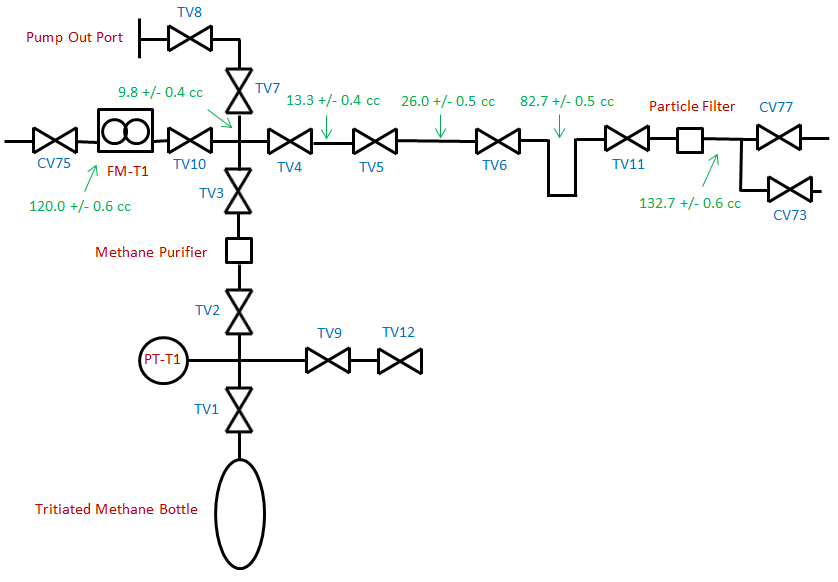
\includegraphics[scale=0.3]{TritiumPlumbingUpdated.png}
\caption{The injection system used in our CH$_3$T calibration technique. CV and TV labels indicate valves in the LUX circulation system and tritium injection system, respectively.  Expansion volumes are labeled in green, and other system components are labeled in red.}
\label{fig:LUXSys}
\end{figure}

\subsection{The zirconium getter}

The LUX gas system uses a hot zirconium getter (SAES-PS4MT15R1) downstream of the CH$_3$T injection system to remove CH$_3$T from the xenon.  Extensive R\&D was conducted using a smaller zirconium getter (SAES-PF4C3R1) at the University of Maryland to learn about the CH$_3$T removal efficiency of these purifiers.  Details of these studies is discussed in section \ref{sec:RD} 